\documentclass{article}
\usepackage[utf8]{inputenc}
\usepackage{tikz}
\usepackage{amsmath}
\usepackage{xcolor}
\usepackage{hyperref}
\usepackage[a4paper, margin=1in]{geometry}
\usetikzlibrary{shapes.geometric, arrows, positioning, fit, backgrounds, matrix, decorations.pathreplacing, chains, calc}

\definecolor{myblue}{RGB}{0, 102, 204}
\definecolor{mygreen}{RGB}{46, 148, 78}
\definecolor{myorange}{RGB}{230, 126, 34}
\definecolor{mypurple}{RGB}{142, 68, 173}
\definecolor{myred}{RGB}{231, 76, 60}

\begin{document}

\title{MSAGAT-Net: Multi-Scale Adaptive Graph Attention Network \\
for Spatiotemporal Forecasting}
\author{Architecture Diagrams}
\date{\today}

\maketitle

\section{Overall Architecture}

\begin{figure}[h]
\centering
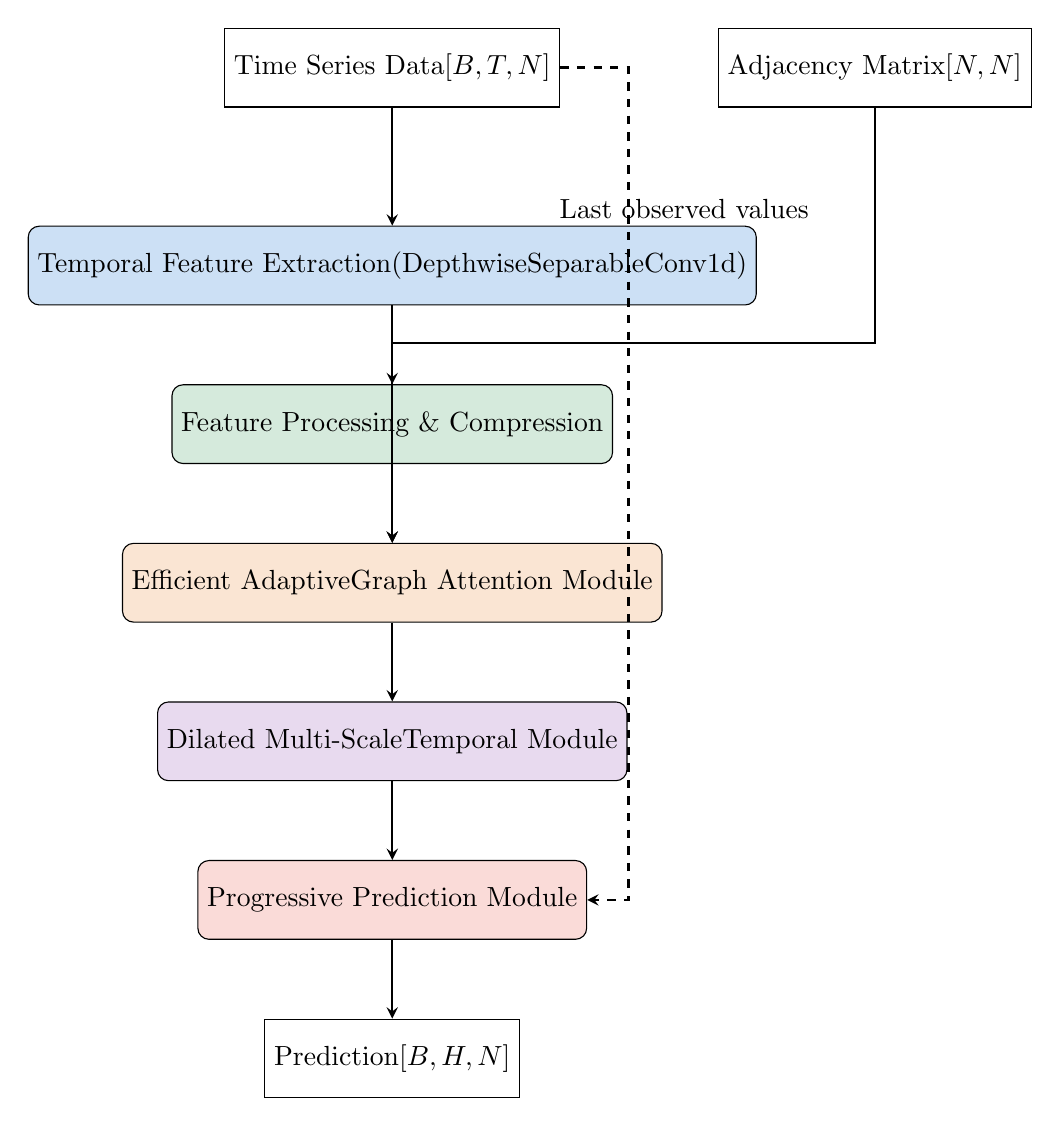
\begin{tikzpicture}[
    node distance=2cm,
    box/.style={rectangle, rounded corners, draw=black, minimum width=3cm, minimum height=1cm, text centered},
    data/.style={rectangle, draw=black, minimum width=3cm, minimum height=1cm, text centered},
    arrow/.style={thick,->,>=stealth}
]

% Input
\node[data] (input) {Time Series Data\\$[B, T, N]$};
\node[data, right=2cm of input] (adj) {Adjacency Matrix\\$[N, N]$};

% Feature extraction
\node[box, below=1.5cm of input, fill=myblue!20] (temporal) {Temporal Feature Extraction\\(DepthwiseSeparableConv1d)};

% Feature processing
\node[box, below=1cm of temporal, fill=mygreen!20] (processing) {Feature Processing \& Compression};

% Main components
\node[box, below=1cm of processing, fill=myorange!20] (graph) {Efficient Adaptive\\ Graph Attention Module};
\node[box, below=1cm of graph, fill=mypurple!20] (multi) {Dilated Multi-Scale\\ Temporal Module};
\node[box, below=1cm of multi, fill=myred!20] (prediction) {Progressive Prediction Module};

% Output
\node[data, below=1cm of prediction] (output) {Prediction\\$[B, H, N]$};

% Arrows
\draw[arrow] (input) -- (temporal);
\draw[arrow] (adj) -- ++(0,-3.5) -| (graph);
\draw[arrow] (temporal) -- (processing);
\draw[arrow] (processing) -- (graph);
\draw[arrow] (graph) -- (multi);
\draw[arrow] (multi) -- (prediction);
\draw[arrow] (prediction) -- (output);

% Last observed value connection
\draw[arrow, dashed] (input) -- ++(3,0) |- (prediction);
\node[right] at ($(input)+(2,-1.8)$) {Last observed values};

\end{tikzpicture}
\caption{Overall architecture of MSAGAT-Net showing the flow from input time series and adjacency matrix to final predictions.}
\end{figure}

\section{Key Components}

\subsection{Temporal Feature Extraction}

\begin{figure}[h]
\centering
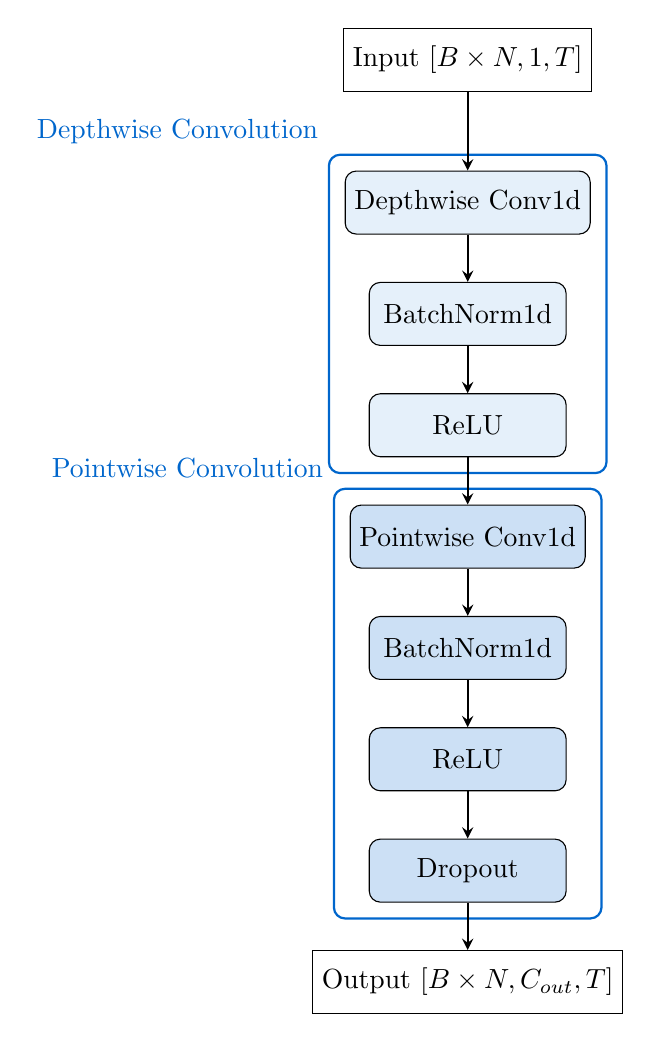
\begin{tikzpicture}[
    node distance=1.8cm,
    box/.style={rectangle, rounded corners, draw=black, minimum width=2.5cm, minimum height=0.8cm, text centered},
    data/.style={rectangle, draw=black, minimum width=2.5cm, minimum height=0.8cm, text centered},
    arrow/.style={thick,->,>=stealth}
]

% Input
\node[data] (input) {Input $[B \times N, 1, T]$};

% Depthwise
\node[box, fill=myblue!10, below=1cm of input] (depthwise) {Depthwise Conv1d};
\node[box, fill=myblue!10, below=0.6cm of depthwise] (bn1) {BatchNorm1d};
\node[box, fill=myblue!10, below=0.6cm of bn1] (relu1) {ReLU};

% Pointwise
\node[box, fill=myblue!20, below=0.6cm of relu1] (pointwise) {Pointwise Conv1d};
\node[box, fill=myblue!20, below=0.6cm of pointwise] (bn2) {BatchNorm1d};
\node[box, fill=myblue!20, below=0.6cm of bn2] (relu2) {ReLU};
\node[box, fill=myblue!20, below=0.6cm of relu2] (dropout) {Dropout};

% Output
\node[data, below=0.6cm of dropout] (output) {Output $[B \times N, C_{out}, T]$};

% Arrows
\draw[arrow] (input) -- (depthwise);
\draw[arrow] (depthwise) -- (bn1);
\draw[arrow] (bn1) -- (relu1);
\draw[arrow] (relu1) -- (pointwise);
\draw[arrow] (pointwise) -- (bn2);
\draw[arrow] (bn2) -- (relu2);
\draw[arrow] (relu2) -- (dropout);
\draw[arrow] (dropout) -- (output);

% Group box for depthwise
\begin{pgfonlayer}{background}
\node[rectangle, draw=myblue, thick, inner sep=0.2cm, rounded corners, fit=(depthwise) (relu1)] (depthwise_group) {};
\node[text=myblue, above left=0cm of depthwise_group.north west] {Depthwise Convolution};
\end{pgfonlayer}

% Group box for pointwise
\begin{pgfonlayer}{background}
\node[rectangle, draw=myblue, thick, inner sep=0.2cm, rounded corners, fit=(pointwise) (dropout)] (pointwise_group) {};
\node[text=myblue, above left=0cm of pointwise_group.north west] {Pointwise Convolution};
\end{pgfonlayer}

\end{tikzpicture}
\caption{Depthwise Separable Convolution for efficient temporal feature extraction.}
\end{figure}

\subsection{Efficient Adaptive Graph Attention Module}

\begin{figure}[h]
\centering
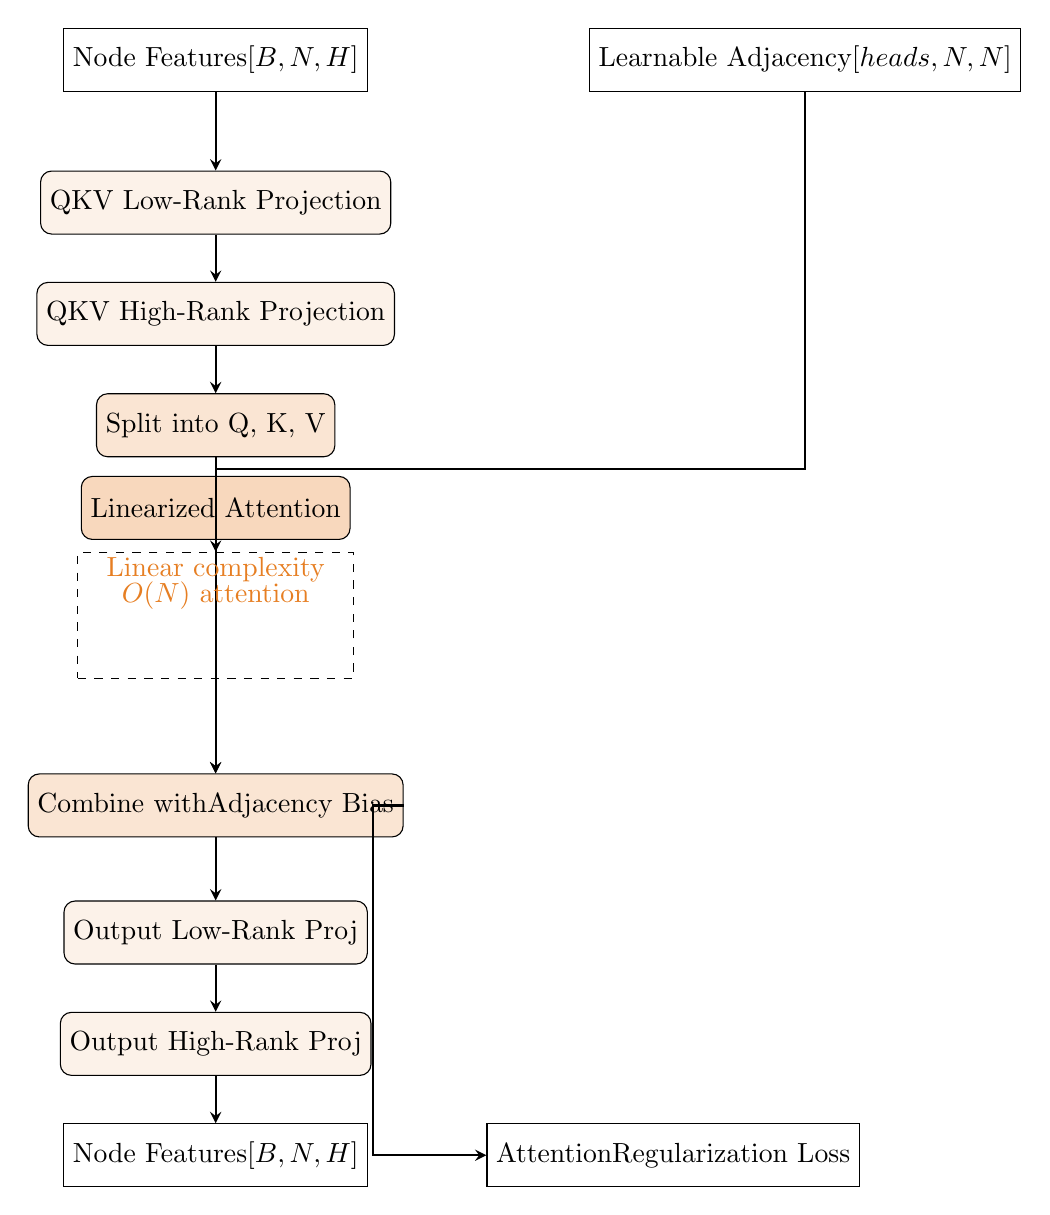
\begin{tikzpicture}[
    node distance=2cm,
    box/.style={rectangle, rounded corners, draw=black, minimum width=2.8cm, minimum height=0.8cm, text centered},
    data/.style={rectangle, draw=black, minimum width=2.8cm, minimum height=0.8cm, text centered},
    proc/.style={rectangle, draw=black, dashed, minimum width=3.5cm, minimum height=1.6cm, text centered},
    arrow/.style={thick,->,>=stealth}
]

% Input
\node[data] (input) {Node Features\\$[B, N, H]$};
\node[data, right=2.8cm of input] (adj) {Learnable Adjacency\\$[heads, N, N]$};

% Low-rank projection
\node[box, fill=myorange!10, below=1cm of input] (qkv_low) {QKV Low-Rank Projection};
\node[box, fill=myorange!10, below=0.6cm of qkv_low] (qkv_high) {QKV High-Rank Projection};

% QKV separation
\node[box, fill=myorange!20, below=0.6cm of qkv_high] (qkv_split) {Split into Q, K, V};

% Attention computation
\node[proc, below=1.2cm of qkv_split] (attn_comp) {};
\node[box, fill=myorange!30, above=0.15cm of attn_comp.north] (linear_attn) {Linearized Attention};

% Combine with adjacency
\node[box, fill=myorange!20, below=1.2cm of attn_comp] (combine) {Combine with\\Adjacency Bias};

% Output projection
\node[box, fill=myorange!10, below=0.8cm of combine] (out_low) {Output Low-Rank Proj};
\node[box, fill=myorange!10, below=0.6cm of out_low] (out_high) {Output High-Rank Proj};

% Output
\node[data, below=0.6cm of out_high] (output) {Node Features\\$[B, N, H]$};
\node[data, right=1.5cm of output] (reg_loss) {Attention\\Regularization Loss};

% Arrows
\draw[arrow] (input) -- (qkv_low);
\draw[arrow] (qkv_low) -- (qkv_high);
\draw[arrow] (qkv_high) -- (qkv_split);
\draw[arrow] (qkv_split) -- (attn_comp);
\draw[arrow] (adj) -- ++(0,-5.2) -| (combine);
\draw[arrow] (attn_comp) -- (combine);
\draw[arrow] (combine) -- (out_low);
\draw[arrow] (out_low) -- (out_high);
\draw[arrow] (out_high) -- (output);
\draw[arrow] (combine) -- ++(2,0) |- (reg_loss);

% Label for attention computation
\node[text=myorange, below=0.1cm of linear_attn] {Linear complexity};
\node[text=myorange, below=0.4cm of linear_attn] {$O(N)$ attention};

\end{tikzpicture}
\caption{Efficient Adaptive Graph Attention Module with linear complexity and low-rank projections.}
\end{figure}

\subsection{Dilated Multi-Scale Temporal Module}

\begin{figure}[h]
\centering
\begin{tikzpicture}[
    node distance=1.5cm,
    box/.style={rectangle, rounded corners, draw=black, minimum width=2.8cm, minimum height=0.8cm, text centered},
    data/.style={rectangle, draw=black, minimum width=2.8cm, minimum height=0.8cm, text centered},
    scale/.style={rectangle, draw=black, rounded corners, fill=mypurple!10, minimum width=2.8cm, minimum height=2cm, text centered},
    arrow/.style={thick,->,>=stealth}
]

% Input
\node[data] (input) {Input Features\\$[B, N, H]$};

% Scale modules
\node[scale, below=1.5cm of input, xshift=-4.5cm] (scale1) {Scale 1\\Dilation = 1\\Conv + BN + ReLU};
\node[scale, right=0.5cm of scale1] (scale2) {Scale 2\\Dilation = 2\\Conv + BN + ReLU};
\node[scale, right=0.5cm of scale2] (scale3) {Scale 3\\Dilation = 4\\Conv + BN + ReLU};
\node[scale, right=0.5cm of scale3] (scale4) {Scale 4\\Dilation = 8\\Conv + BN + ReLU};

% Fusion
\node[box, fill=mypurple!30, below=1.5cm of input] (fusion) {Adaptive Scale Fusion};
\node[box, fill=mypurple!20, below=0.6cm of fusion] (fusion_low) {Fusion Low-Rank Proj};
\node[box, fill=mypurple!20, below=0.6cm of fusion_low] (fusion_high) {Fusion High-Rank Proj};
\node[box, fill=mypurple!20, below=0.6cm of fusion_high] (layernorm) {LayerNorm + Residual};

% Output
\node[data, below=0.6cm of layernorm] (output) {Output Features\\$[B, N, H]$};

% Arrows
\draw[arrow] (input) -- ++(0,-0.75) -| (scale1.north);
\draw[arrow] (input) -- ++(0,-0.75) -| (scale2.north);
\draw[arrow] (input) -- ++(0,-0.75) -| (scale3.north);
\draw[arrow] (input) -- ++(0,-0.75) -| (scale4.north);

\draw[arrow] (scale1.south) -- ++(0,-0.5) -| (fusion.north);
\draw[arrow] (scale2.south) -- ++(0,-0.5) -| (fusion.north);
\draw[arrow] (scale3.south) -- ++(0,-0.5) -| (fusion.north);
\draw[arrow] (scale4.south) -- ++(0,-0.5) -| (fusion.north);

\draw[arrow] (fusion) -- (fusion_low);
\draw[arrow] (fusion_low) -- (fusion_high);
\draw[arrow] (fusion_high) -- (layernorm);
\draw[arrow] (layernorm) -- (output);

% Residual connection
\draw[arrow, dashed] (fusion) -- ++(3.5,0) |- (layernorm);

\end{tikzpicture}
\caption{Dilated Multi-Scale Temporal Module with adaptive fusion of features from different time scales.}
\end{figure}

\subsection{Progressive Prediction Module}

\begin{figure}[h]
\centering
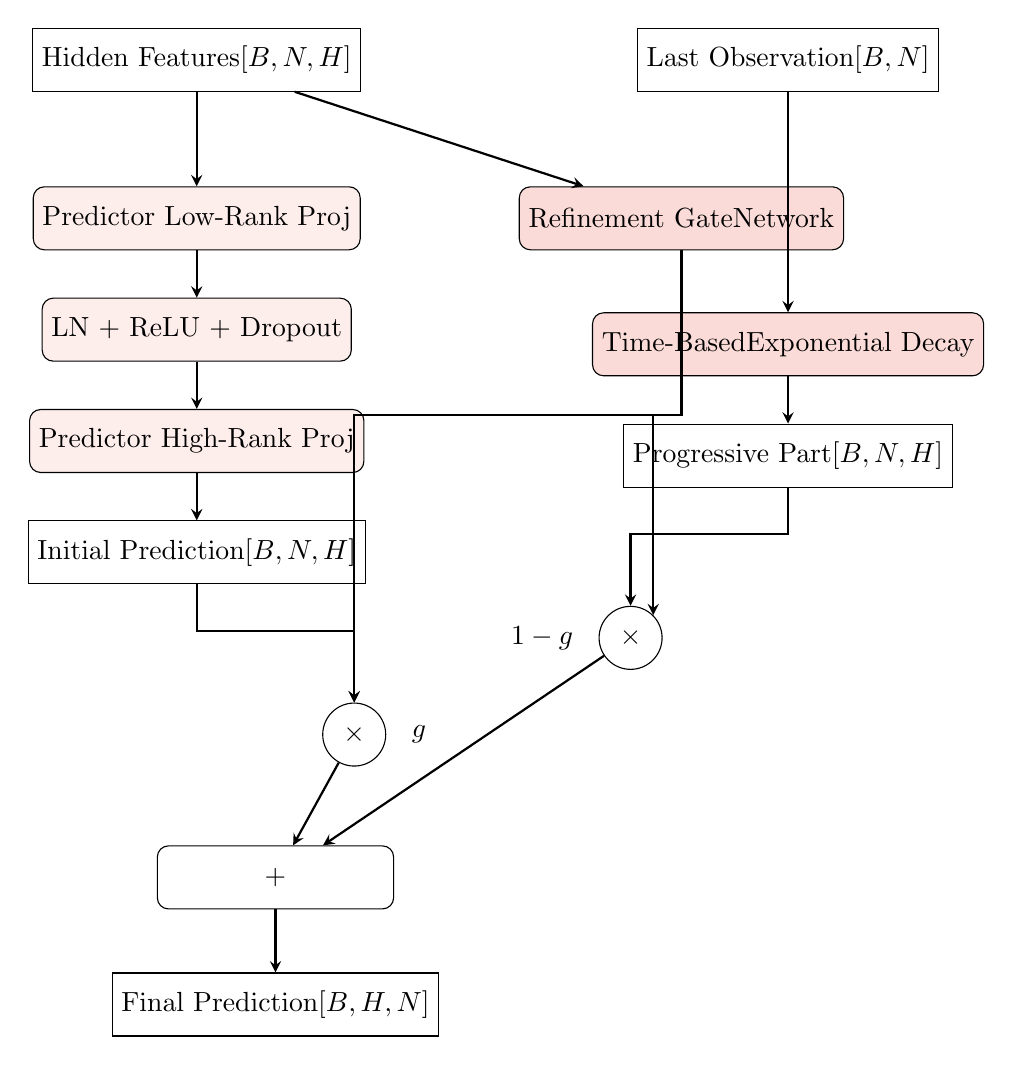
\begin{tikzpicture}[
    node distance=1.5cm,
    box/.style={rectangle, rounded corners, draw=black, minimum width=3cm, minimum height=0.8cm, text centered},
    data/.style={rectangle, draw=black, minimum width=3cm, minimum height=0.8cm, text centered},
    gate/.style={circle, draw=black, minimum size=0.8cm, text centered},
    arrow/.style={thick,->,>=stealth}
]

% Inputs
\node[data] (input) {Hidden Features\\$[B, N, H]$};
\node[data, right=3.5cm of input] (last) {Last Observation\\$[B, N]$};

% Prediction pathway
\node[box, fill=myred!10, below=1.2cm of input] (pred_low) {Predictor Low-Rank Proj};
\node[box, fill=myred!10, below=0.6cm of pred_low] (pred_mid) {LN + ReLU + Dropout};
\node[box, fill=myred!10, below=0.6cm of pred_mid] (pred_high) {Predictor High-Rank Proj};
\node[data, below=0.6cm of pred_high] (init_pred) {Initial Prediction\\$[B, N, H]$};

% Refinement pathway
\node[box, fill=myred!20, below right=1.2cm and 2cm of input] (refine_gate) {Refinement Gate\\Network};
\node[box, fill=myred!20, below=2.8cm of last] (time_decay) {Time-Based\\Exponential Decay};
\node[data, below=0.6cm of time_decay] (prog_part) {Progressive Part\\$[B, N, H]$};

% Gating mechanism
\node[gate, below=1.5cm of init_pred, xshift=2cm] (gate) {$\times$};
\node[gate, below=1.5cm of prog_part, xshift=-2cm] (gate2) {$\times$};
\node[box, below=1cm of gate, xshift=-1cm] (add) {$+$};

% Output
\node[data, below=0.8cm of add] (output) {Final Prediction\\$[B, H, N]$};

% Arrows
\draw[arrow] (input) -- (pred_low);
\draw[arrow] (pred_low) -- (pred_mid);
\draw[arrow] (pred_mid) -- (pred_high);
\draw[arrow] (pred_high) -- (init_pred);

\draw[arrow] (input) -- (refine_gate);
\draw[arrow] (last) -- (time_decay);
\draw[arrow] (time_decay) -- (prog_part);

\draw[arrow] (init_pred) -- ++(0,-1) -| (gate);
\draw[arrow] (refine_gate) -- ++(0,-2.5) -| (gate);
\draw[arrow] (refine_gate) -- ++(0,-2.5) -| (gate2.north east);
\draw[arrow] (prog_part) -- ++(0,-1) -| (gate2);

\draw[arrow] (gate) -- (add);
\draw[arrow] (gate2) -- (add);
\draw[arrow] (add) -- (output);

% Gate labels
\node[right=0.2cm of gate] {$g$};
\node[left=0.2cm of gate2] {$1-g$};

\end{tikzpicture}
\caption{Progressive Prediction Module with adaptive gating and time-decay refinement.}
\end{figure}

\section{Detailed Data Flow}

\begin{figure}[h]
\centering
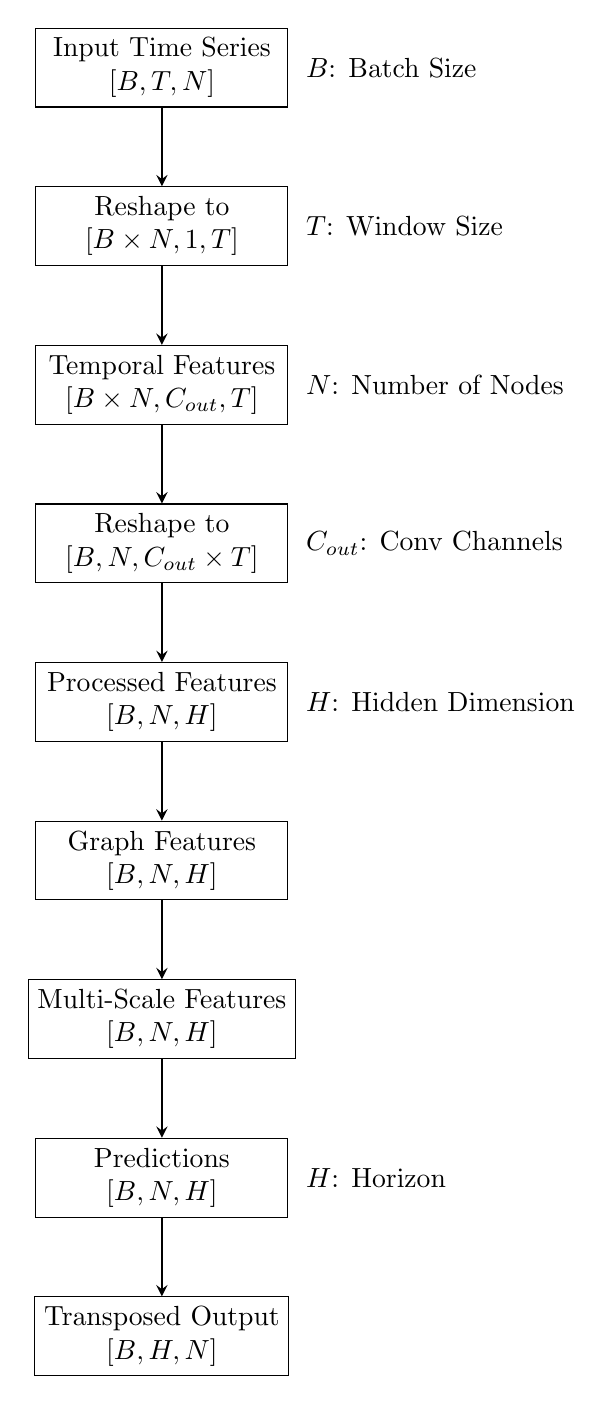
\begin{tikzpicture}[
    node distance=2cm,
    data/.style={rectangle, draw=black, minimum width=3.2cm, minimum height=1cm, text centered, align=center},
    arrow/.style={thick,->,>=stealth}
]

% Input format
\node[data] (input) {Input Time Series\\$[B, T, N]$};

% Data reshaping
\node[data, below=1cm of input] (reshape) {Reshape to\\$[B \times N, 1, T]$};

% Temporal features
\node[data, below=1cm of reshape] (temp_feat) {Temporal Features\\$[B \times N, C_{out}, T]$};

% Reshaping back
\node[data, below=1cm of temp_feat] (reshape2) {Reshape to\\$[B, N, C_{out} \times T]$};

% Feature processing
\node[data, below=1cm of reshape2] (process) {Processed Features\\$[B, N, H]$};

% Graph features
\node[data, below=1cm of process] (graph) {Graph Features\\$[B, N, H]$};

% Temporal fusion
\node[data, below=1cm of graph] (temporal) {Multi-Scale Features\\$[B, N, H]$};

% Prediction
\node[data, below=1cm of temporal] (pred) {Predictions\\$[B, N, H]$};

% Output
\node[data, below=1cm of pred] (output) {Transposed Output\\$[B, H, N]$};

% Arrows
\draw[arrow] (input) -- (reshape);
\draw[arrow] (reshape) -- (temp_feat);
\draw[arrow] (temp_feat) -- (reshape2);
\draw[arrow] (reshape2) -- (process);
\draw[arrow] (process) -- (graph);
\draw[arrow] (graph) -- (temporal);
\draw[arrow] (temporal) -- (pred);
\draw[arrow] (pred) -- (output);

% Labels
\node[right=0.1cm of input] {$B$: Batch Size};
\node[right=0.1cm of reshape] {$T$: Window Size};
\node[right=0.1cm of temp_feat] {$N$: Number of Nodes};
\node[right=0.1cm of reshape2] {$C_{out}$: Conv Channels};
\node[right=0.1cm of process] {$H$: Hidden Dimension};
\node[right=0.1cm of graph] {};
\node[right=0.1cm of temporal] {};
\node[right=0.1cm of pred] {$H$: Horizon};

\end{tikzpicture}
\caption{Detailed data flow through the MSAGAT-Net architecture showing tensor shapes at each step.}
\end{figure}

\end{document}